\documentclass{scrartcl}
\usepackage[utf8]{inputenc}
\usepackage{tikz}
\usetikzlibrary{arrows,decorations.pathmorphing,backgrounds,fit,positioning,shapes.symbols,chains,shapes.geometric,shapes.arrows,calc}

\begin{document}
  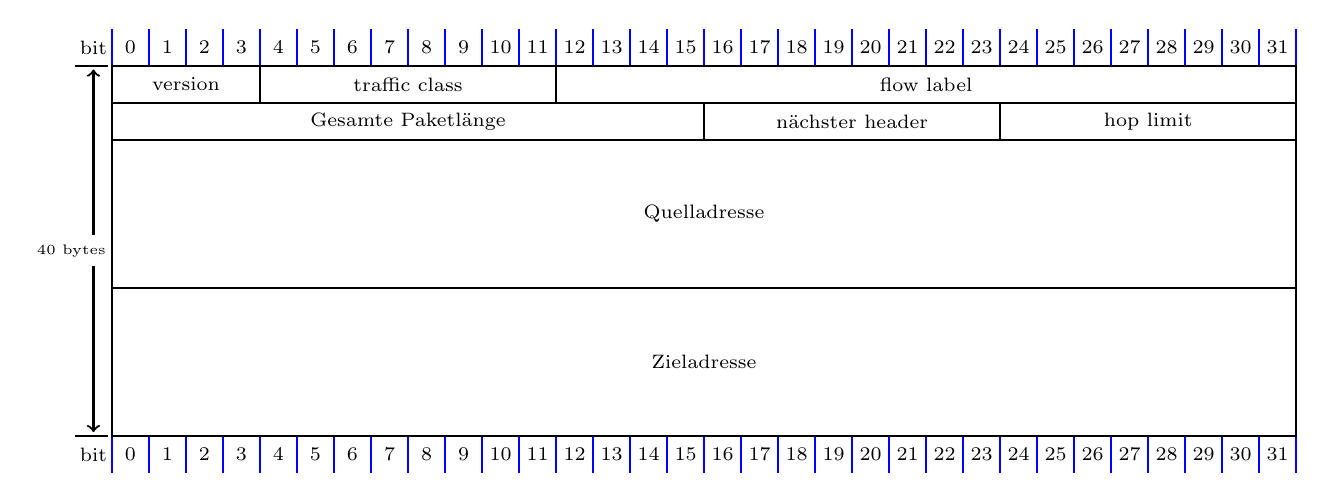
\begin{tikzpicture}[scale=0.47]
	\foreach \x in {0,...,31}
		\node at (\x+0.5,20.5) {\scriptsize \x};
	\foreach \x in {0,...,31}
		\node at (\x+0.5,9.5) {\scriptsize \x};
	\foreach \x in {0,...,32}
		\draw[thick, blue] (\x,9) -- (\x,21);
	\node[thick] (bit1) at (-0.5,20.5) {\scriptsize bit};
	\node[thick] (bit2) at (-0.5,9.5) {\scriptsize bit};
	\draw [<->, thick] (-0.5, 19.9) -- (-0.5,10.1);
	\draw [thick] (-1, 20) -- (-0.1,20);
	\draw [thick] (-1, 10) -- (-0.1,10);
	\node[fill=white] at (-1.1,15) {\tiny 40 bytes};
	\filldraw[thick,draw=black, fill=white] (0,20) rectangle (4,19); \node (mode) at (2,19.5) {\scriptsize version};
	\filldraw[thick,draw=black, fill=white] (4,20) rectangle (12,19); \node (mode) at (8,19.5) {\scriptsize traffic class};
	\filldraw[thick,draw=black, fill=white] (12,20) rectangle (32,19); \node (mode) at (22,19.5) {\scriptsize flow label};
	\filldraw[thick,draw=black, fill=white] (0,19) rectangle (16,18); \node (mode) at (8,18.5) {\scriptsize Gesamte Paketlänge};
	\filldraw[thick,draw=black, fill=white] (16,19) rectangle (24,18); \node (mode) at (20,18.5) {\scriptsize nächster header};
	\filldraw[thick,draw=black, fill=white] (24,19) rectangle (32,18); \node (mode) at (28,18.5) {\scriptsize hop limit};
	\filldraw[thick,draw=black, fill=white] (0,18) rectangle (32,14); \node (mode) at (16,16) {\scriptsize Quelladresse};
	\filldraw[thick,draw=black, fill=white] (0,14) rectangle (32,10); \node (mode) at (16,12) {\scriptsize Zieladresse};
	\end{tikzpicture}
\end{document}
